\documentclass{article}
\setlength{\parskip}{5pt} % esp. entre parrafos
\setlength{\parindent}{0pt} % esp. al inicio de un parrafo
\usepackage{listings} % listings
\usepackage{color} %colores
\usepackage{amsmath} % mates
\usepackage[sort&compress,numbers]{natbib} % referencias
\usepackage{url} % que las URLs se vean lindos
\usepackage[top=15mm,left=20mm,right=20mm,bottom=25mm]{geometry} % margenes 
\usepackage{hyperref} % ligas de URLs
\usepackage{graphicx} % poner figuras
\usepackage[spanish]{babel} % otros idiomas


\author{Claudia Lizeth Hern\'andez Ram\'irez} % author
\title{Homework 11 - Frentes de Pareto} % titulo
\date{\today}

\definecolor{myfucsia}{rgb}{1, 0.078, 0.576}
\definecolor{mygray}{rgb}{0.752, 0.752, 0.752}
\definecolor{mypurple}{rgb}{0.580, 0, 0.827}
\lstset{ 
  backgroundcolor=\color{mygray},
  commentstyle=\color{myfucsia},
  keywordstyle=\color{mypurple}, 
  numberstyle=\tiny\color{myfucsia}
  stringstyle=\color{mypurple}, 
  breaklines=true,
}


\begin{document} % inicia contenido

\maketitle % cabecera



% INTRODUCCIOOOOOOOOOOOON
\section{Introducci\'{o}n}\label{intro} % seccion y etiqueta
Grafica el porcentaje de soluciones de Pareto como funci\'on del n\'umero de funciones objetivo con diagramas de viol\'in combinados con diagramas de caja-bigote, verificando que diferencias observadas, cuando las haya, sean estad\'isticamente significativas. Razona en escrito a qu\'e se debe el comportamiento observado.


% DESARROLLOOOOOOOOOOOO
\section{Desarrollo}\label{desarrollo} % Desarrollo de la tarea

Inici\'e trabajando con uno de los c\'odigos vistos en clase \citep{Parfronts}, agregando dos ciclos \texttt{FOR} con los que se variar\'ian las funciones objetivo y se realizar\'ian las iteraciones.

\begin{lstlisting}[language=R, caption= Segmento de c\'odigo ciclos \texttt{FOR} y definici\'on de variables.]
vc <- 4 #Cuantas variables
md <- 3 #Grado maximo
tc <- 5#Cuantos terminos
funobj = c(2, 3, 4, 5) #Funciones objetivo para k(2, 3, 4, 5)
replicaa = 1:20
for (k in funobj) {
  for (reply in replicaa) {
\end{lstlisting}


Posteriormente, utilizando como base el c\'odigos que se encuentra en el repositorio de Schaeffer \citep{Violin} y con ayuda del art\'iculo\citep{ggplotaest}, gener\'e la figura \ref{Figura 1}.
\begin{lstlisting}[language=R, caption= Segmento de c\'odigo gr\'afica.]
    datos$k = as.factor(datos$k)
    gr = ggplot(datos, aes(x = k, y = porcentaje)) +
      geom_violin(fill = "#C1B3D7", color = "#A589C1")
    gr + geom_boxplot(width = 0.1, fill = "#A5DEEE",
                      color = "black", lwd = 0.3)+
      theme(panel.background = element_rect(fill = "#FDDEEE",
                                            color = "black")) +
      labs(x = "N\'umero de funciones objetivo",
           y = "Porcentaje de soluciones Pareto")
\end{lstlisting}
\newpage

Como es costumbre, realic\'e pruebas estad\'isticas a mis resultados, los resultados se encuentran en la secci\'on de \texttt{Estad\'istica}.
\begin{lstlisting}[language=R, caption= Segmento de c\'odigo pruebas estad\'isticas.]
#Estad\'isitica prueba de normalidad - 
    #con p menor a 0.05 se rechaza hipotesis nula H0
    #H0: los datos proceden de una distribuci\'on normal
    #H1: los datos no proceden de una distribuci\'on normal
tapply(datos$porcentaje, datos$k, shapiro.test)

#PRUEBA ESTADISTICA
datos%>%
  group_by(k) %>%
  summarise(
    cantidad_de_participantes = n(),
    promedio = mean(porcentaje, na.rm = TRUE),
    desviacion_estandar = sd(porcentaje, na.rm = TRUE),
    varianza = sd(porcentaje, na.rm = TRUE)^2,
    mediana = median(porcentaje, na.rm = TRUE),
    rango_intercuartil =  IQR(porcentaje, na.rm = TRUE)
  )

kruskal.test(porcentaje ~ k, data = datos)
pairwise.wilcox.test(datos$porcentaje, datos$k)
\end{lstlisting}




\section{Estad\'istica}
\begin{table}[ht]
    \centering
    \caption{Resultados obtenidos de prueba de normalidad de Shapiro.} 
    \begin{tabular}{|c|c|c|c|}
    \hline
    K & W value & P value & ¿Se acepta H0?  \\
    \hline
    2 & 0.7083 & $4.93\times 10^{-5}$ & no \\
    \hline 
    3 & 0.6697 & $1.70\times 10^{-5}$ & no  \\
    \hline 
    4 & 0.9580 & 0.5052 & s\'i \\
    \hline
    5 & 0.9097 & 0.0631 & s\'i \\
    \hline 
\end{tabular}
    \label{cuadro 1}
\end{table}

\begin{table}[ht]
    \centering
    \caption{Resultados obtenidos de prueba Kruskal-Wallis.} 
    \begin{tabular}{|c|c|c|}
    \hline
    Chi cuadrada & DF & P  \\
    \hline
    47.786 & 3 & $2.365\times 10^{-10}$ \\
    \hline
\end{tabular}
    \label{cuadro 2}
\end{table}

\begin{table}[htb]
    \centering
    \caption{Diferencias entre grupos. Paiwise Wilcox.} 
    \begin{tabular}{|c|c|c|c|c|}
    \hline
    "" & 2 & 3 & 4 \\
    \hline
    3 & 0.00035 & "" & "" \\
    \hline
    4 & $1.2\times 10^{-6}$ & 0.00324  & "" \\
    \hline
    5 & $5.3\times 10^{-7}$ & 0.00035 & 0.33680 \\
    \hline
    \end{tabular}
    \label{cuadro 3}
\end{table}

\begin{table}[htb]
    \centering
    \caption{Informaci\'on individual de los datos.} 
    \begin{tabular}{|c|c|c|c|c|c|c|}
    \hline
    Carga & Qty. Participantes & promedio & Desv. Std. & Varianza & Mediana & Rango Intercuartil  \\
    \hline
    2 & 20 & 2.72 & 2.84 & 8.07 & 1.75 & 2.0 \\
    \hline
    3 & 20 & 17.00 & 22.70 & 515.00 & 6.75 & 14.4 \\
    \hline
    4 & 20 & 37.80 & 22.30 & 496.00 & 39 & 34.1 \\
    \hline
    5 & 20 & 48.80 & 29.80 & 887.00 & 42.2 & 56.0 \\
    \hline
\end{tabular}
    \label{cuadro 4}
\end{table}

\begin{figure}[htb!] % figura
    \centering
    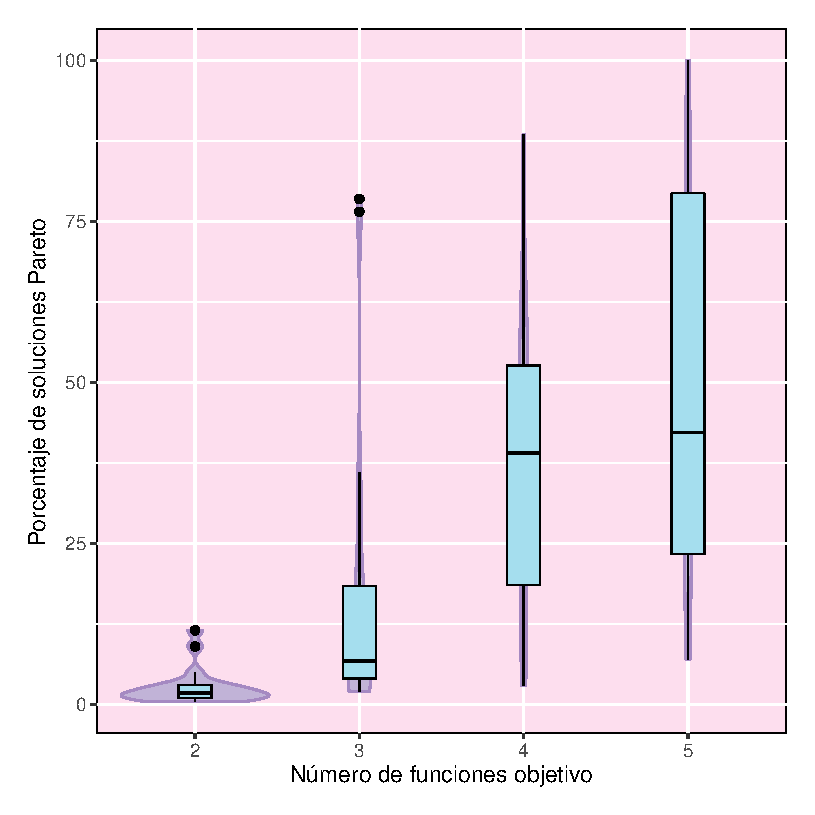
\includegraphics[width=100mm]{HW11.eps} % archivo
    \caption{Porcentaje de soluciones de Pareto vs Funci\'on objetivo.}
    \label{Figura 1}
\end{figure}
\newpage

%CONCLUSIOOOON
\section{Conclusi\'on}
Como se puede observar en la figura \ref{Figura 1}, el aumento en el porcentaje de soluciones de Pareto, depende fuertemente del n\'umero de funciones objetivo que se tengan.\newline Entre menos funciones objetivo se tengan, el porcentaje de Pareto ser\'a menor; Por otro lado, mientras mas funciones objetivo se tengan, el porcentaje de Pareto aumenta hasta lograr una optimizaci\'on de casi el 100\%.
Se puede esta relaci\'on se puede explicar en base a que, como se tiene una mayor cantidad de funciones para optimizar, si bien no estar\'an optimizadas en todos los criterios, lo estar\'an para algunos otros, satisfaciendo as\'i a por lo menos alguna de las otras funciones.\newline
Esto se comprueba con las pruebas estad\'isticas que se aplicaron, ya que con una \texttt{P = $2.365\times 10^{-10}$} se rechaza la hip\'otesis nula, lo cual nos indica que existen diferencias significativas entre las funciones objetivo.

% BIBLIOGRAFIAAAAAAS
\bibliography{referencias}
\bibliographystyle{plainnat}
\end{document}


